\model{Math Methods}

Consider the following methods defined in the \java{Math} class:

\begin{javalst}
    public static int abs(int a)
    public static double log(double a)
    public static double pow(double a, double b)
    public static double random()
    public static int subtractExact(int x, int y)
\end{javalst}

Note this list isn't exhaustive; \java{Math} has over 70 methods in total.
To invoke methods from another class (like \java{Math}), you must first specify the class name:

\begin{javalst}
    value = abs(-5);       // Error: cannot find symbol
    value = Math.abs(-5);  // correct
\end{javalst}

The period in this example is called the \emph{dot operator}. When reading the above code out loud, you would say ``math dot abs''.

Here is the Java documentation for the methods listed above:
\nopagebreak
\begin{center}
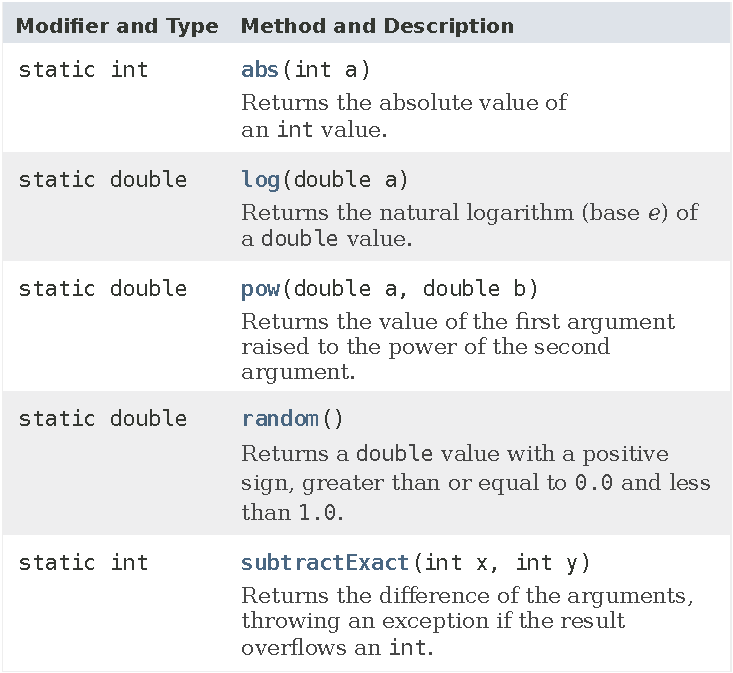
\includegraphics[scale=0.90]{math-javadoc.pdf}
\end{center}


\quest{15 min}


\Q What type of value does \java{Math.random()} return? Give an example of what it would look like.

\begin{answer}
It returns a random \texttt{double} value greater than or equal to 0.0 and less than 1.0.
For example, the value 0.7851637186510342.
\end{answer}


\Q When \emph{invoking} a method, what do you need to specify before and after the method name?

\begin{answer}
Before the name, you need to specify the class name (unless the method is in the same class).
After the name, you need to specify the required values.
\end{answer}


\Q For each method, write a Java statement that invokes it and assigns the result to a variable.

\begin{answer}[8em]
\vspace{-1ex}
\begin{javaans}
answer = Math.abs(-5);
length = Math.log(1.2);
amount = Math.pow(3.4, 5.6);
number = Math.random();
result = Math.subtractExact(-78, 90);
\end{javaans}
\end{answer}


\Q When \emph{defining} a method, what do you need to specify before and after the method name?

\begin{answer}
Before the name, you need to specify what type of value the method will return.
After the name, you need to specify what values are required to invoke the method.
\end{answer}


\Q Define a method named \java{average} that requires two integers \java{x} and \java{y} and returns a \java{double}. (Don't write any semicolons or braces.)

\begin{answer}
\begin{javaans}
public static double average(int x, int y)
\end{javaans}
\end{answer}


\comment{
What you wrote for the previous question is called the method's \textbf{signature}.
The variables declared inside the parentheses are called \textbf{parameters}.
When invoking the method, the values you provide are called \textbf{arguments}.
Since arguments will be assigned to parameters, their types must be compatible.
}


\Q How many parameters and arguments does each method have?

\begin{center}
\begin{tabular}{|c|C{1in}|C{1in}|}
\hline
\tr Method & \tr \# Params & \tr \# Args \\
\hline
\java{abs} & \ans{1} & \ans{1} \\
\hline
\java{log} & \ans{1} & \ans{1} \\
\hline
\java{pow} & \ans{2} & \ans{2} \\
\hline
\java{random} & \ans{0} & \ans{0} \\
\hline
\java{subtractExact} & \ans{2} & \ans{2} \\
\hline
\java{println} & \ans{1} & \ans{1} \\
\hline
\end{tabular}
\end{center}


\Q Consider the statement \java{System.out.println("Price: " + price);} where the value of \java{price} is 9.99. What is the argument that \texttt{println} receives?

\begin{answer}
\begin{javaans}
"Price: 9.99"
\end{javaans}
\end{answer}


\Q Consider the statement \java{System.out.printf("Price: \%f", price);} where the value of \java{price} is 9.99. Why does \java{println} use \emph{plus} and \java{printf} use \emph{comma} to specify the arguments?

\begin{answer}[5em]
The \java{println} method requires only one argument, so plus in this context means concatenate.
The \java{printf} method requires multiple arguments: one for the format string, and others for the values to substitute.
\end{answer}
